\pdfminorversion=4 % for acroread
\documentclass[aspectratio=169,t,xcolor={usenames,dvipsnames}]{beamer}
%\documentclass[t,handout,xcolor={usenames,dvipsnames}]{beamer}
\usepackage{../beamerstyle}
\usepackage{dsfont}
\usepackage{bm}
\usepackage[english]{babel}
\usepackage[utf8]{inputenc}
\usepackage{graphicx}
\usepackage{algorithm}
\usepackage[ruled,vlined,algo2e,linesnumbered]{algorithm2e}
%\usepackage[boxed,vlined]{algorithm2e}
\usepackage{hyperref}
\usepackage{booktabs}
\usepackage{mathtools}

\usepackage{amsmath,amssymb}
\usepackage{listings}
\lstset{frame=lines,framesep=3pt,numbers=left,numberblanklines=false,basicstyle=\ttfamily\small}

\usepackage{subfig}
\usepackage{multicol}
%\usepackage{appendixnumberbeamer}
%
\usepackage{tcolorbox}

\usepackage{pgfplots}
\usepackage{tikz}
\usetikzlibrary{trees} 
\usetikzlibrary{shapes.geometric}
\usetikzlibrary{positioning,shapes,shadows,arrows,calc,mindmap}
\usetikzlibrary{positioning,fadings,through}
\usetikzlibrary{decorations.pathreplacing}
\usetikzlibrary{intersections}
\usetikzlibrary{positioning,fit,calc,shadows,backgrounds}
\pgfdeclarelayer{background}
\pgfdeclarelayer{foreground}
\pgfsetlayers{background,main,foreground}
\tikzstyle{activity}=[rectangle, draw=black, rounded corners, text centered, text width=8em]
\tikzstyle{data}=[rectangle, draw=black, text centered, text width=8em]
\tikzstyle{myarrow}=[->, thick, draw=black]

% Define the layers to draw the diagram
\pgfdeclarelayer{background}
\pgfdeclarelayer{foreground}
\pgfsetlayers{background,main,foreground}

%\usepackage{listings}
%\lstset{numbers=left,
%  showstringspaces=false,
%  frame={tb},
%  captionpos=b,
%  lineskip=0pt,
%  basicstyle=\ttfamily,
%%  extendedchars=true,
%  stepnumber=1,
%  numberstyle=\small,
%  xleftmargin=1em,
%  breaklines
%}

 
\definecolor{blue}{RGB}{0, 74, 153}

\usetheme{Boadilla}
%\useinnertheme{rectangles}
\usecolortheme{whale}
\setbeamercolor{alerted text}{fg=blue}
\useoutertheme{infolines}
\setbeamertemplate{navigation symbols}{\vspace{-5pt}} % to lower the logo
\setbeamercolor{date in head/foot}{bg=blue} % blue
\setbeamercolor{date in head/foot}{fg=white}
\setbeamercolor{author in head/foot}{bg=blue} %blue
\setbeamercolor{title in head/foot}{bg=blue} % blue
\setbeamercolor{title}{fg=white, bg=blue}
\setbeamercolor{block title}{fg=white,bg=blue}
\setbeamercolor{block body}{bg=blue!10}
\setbeamercolor{frametitle}{fg=white, bg=blue}
\setbeamercovered{invisible}

\makeatletter
\setbeamertemplate{footline}
{
  \leavevmode%
  \hbox{%
  \begin{beamercolorbox}[wd=.333333\paperwidth,ht=2.25ex,dp=1ex,center]{author in head/foot}%
    \usebeamerfont{author in head/foot}\insertshortauthor
  \end{beamercolorbox}%
  \begin{beamercolorbox}[wd=.333333\paperwidth,ht=2.25ex,dp=1ex,center]{title in head/foot}%
    \usebeamerfont{title in head/foot}\insertshorttitle
  \end{beamercolorbox}%
  \begin{beamercolorbox}[wd=.333333\paperwidth,ht=2.25ex,dp=1ex,right]{date in head/foot}%
    \usebeamerfont{date in head/foot}Week \@week, Topic \@topicnumber, Slide \insertframenumber{}\hspace*{2em}
%    \insertframenumber\hspace*{2ex} 
  \end{beamercolorbox}}%
  \vskip0pt%
}

\newcommand{\@week}{0}
\newcommand{\@topicnumber}{0}
\newcommand{\week}[1]{\renewcommand{\@week}{#1}}
\newcommand{\topicnumber}[1]{\renewcommand{\@topicnumber}{#1}}

\makeatother

%\pgfdeclareimage[height=1.2cm]{automl}{images/logos/automl.png}
%\pgfdeclareimage[height=1.2cm]{freiburg}{images/logos/freiburg}

%\logo{\pgfuseimage{freiburg}}

\input{../latex_main/macros}




\newcommand{\inducer}{\mathcal{I}}
\newcommand{\R}{\mathds{R}}

%The following might look confusing but allows us to switch the notation of the optimization problem independently from the notation of the hyper parameter optimization
\newcommand{\xx}{\conf} %x of the optimizer
\newcommand{\xxi}[1][i]{\conf_{#1}} %i-th component of xx (not confuse with i-th individual)
\newcommand{\XX}{\pcs} %search space / domain of f
\newcommand{\f}{\cost} %objective function

\newenvironment{blocki}[1] % itemize block
{
 \begin{block}{#1}\begin{itemize}
}
{
\end{itemize}\end{block}
}

\title[AutoML: Hyperparameter Optimization]{AutoML: Hyperparameter Optimization}
%\subtitle{Overview for this Week} %To be defined in source!
%TODO: change authors!
\author[Jakob Richter]{Bernd Bischl \and Frank Hutter \and Lars Kotthoff\newline \and Marius Lindauer}
\institute{}
\date{}


\usepackage[normalem]{ulem}
\usepackage{pifont}
\usepackage{relsize}
\renewcommand{\lit}[1]{{\smaller\color{black!60}[#1]}}
\title[AutoML: Practical]{AutoML: Practical Considerations} 
\subtitle{Introduction}
\author[Janek Thomas]{Bernd Bischl \and Frank Hutter \and Lars Kotthoff\newline \and Marius Lindauer \and \underline{Janek Thomas} \and Joaquin Vanschoren}

\begin{document}

\maketitle


%----------------------------------------------------------------------
%----------------------------------------------------------------------

\begin{frame}{From HPO to AutoML}
  So far we covered
  \begin{itemize}
    \item HPO as black-box optimization
    \begin{itemize}
      \item Grid- and random search, EAs, BO
    \end{itemize}
    \item Speedup techniques for HPO
    \begin{itemize}
      \item Multi-fidelity, meta-learning, ...
    \end{itemize}
    \item Multi-objective HPO
    \begin{itemize}
      \item NSGA-II, ParEGO, ...
    \end{itemize}
    \item Neural Architecture Search (NAS)
    \begin{itemize}
      \item One-Shot approaches, DARTS, ...
    \end{itemize}
  \end{itemize}
  
  \vspace{1cm}

  $\longrightarrow$ So far we haven't talked (much) about practical considerations.

\end{frame}

\begin{frame}{From HPO to AutoML}
    \begin{center}
      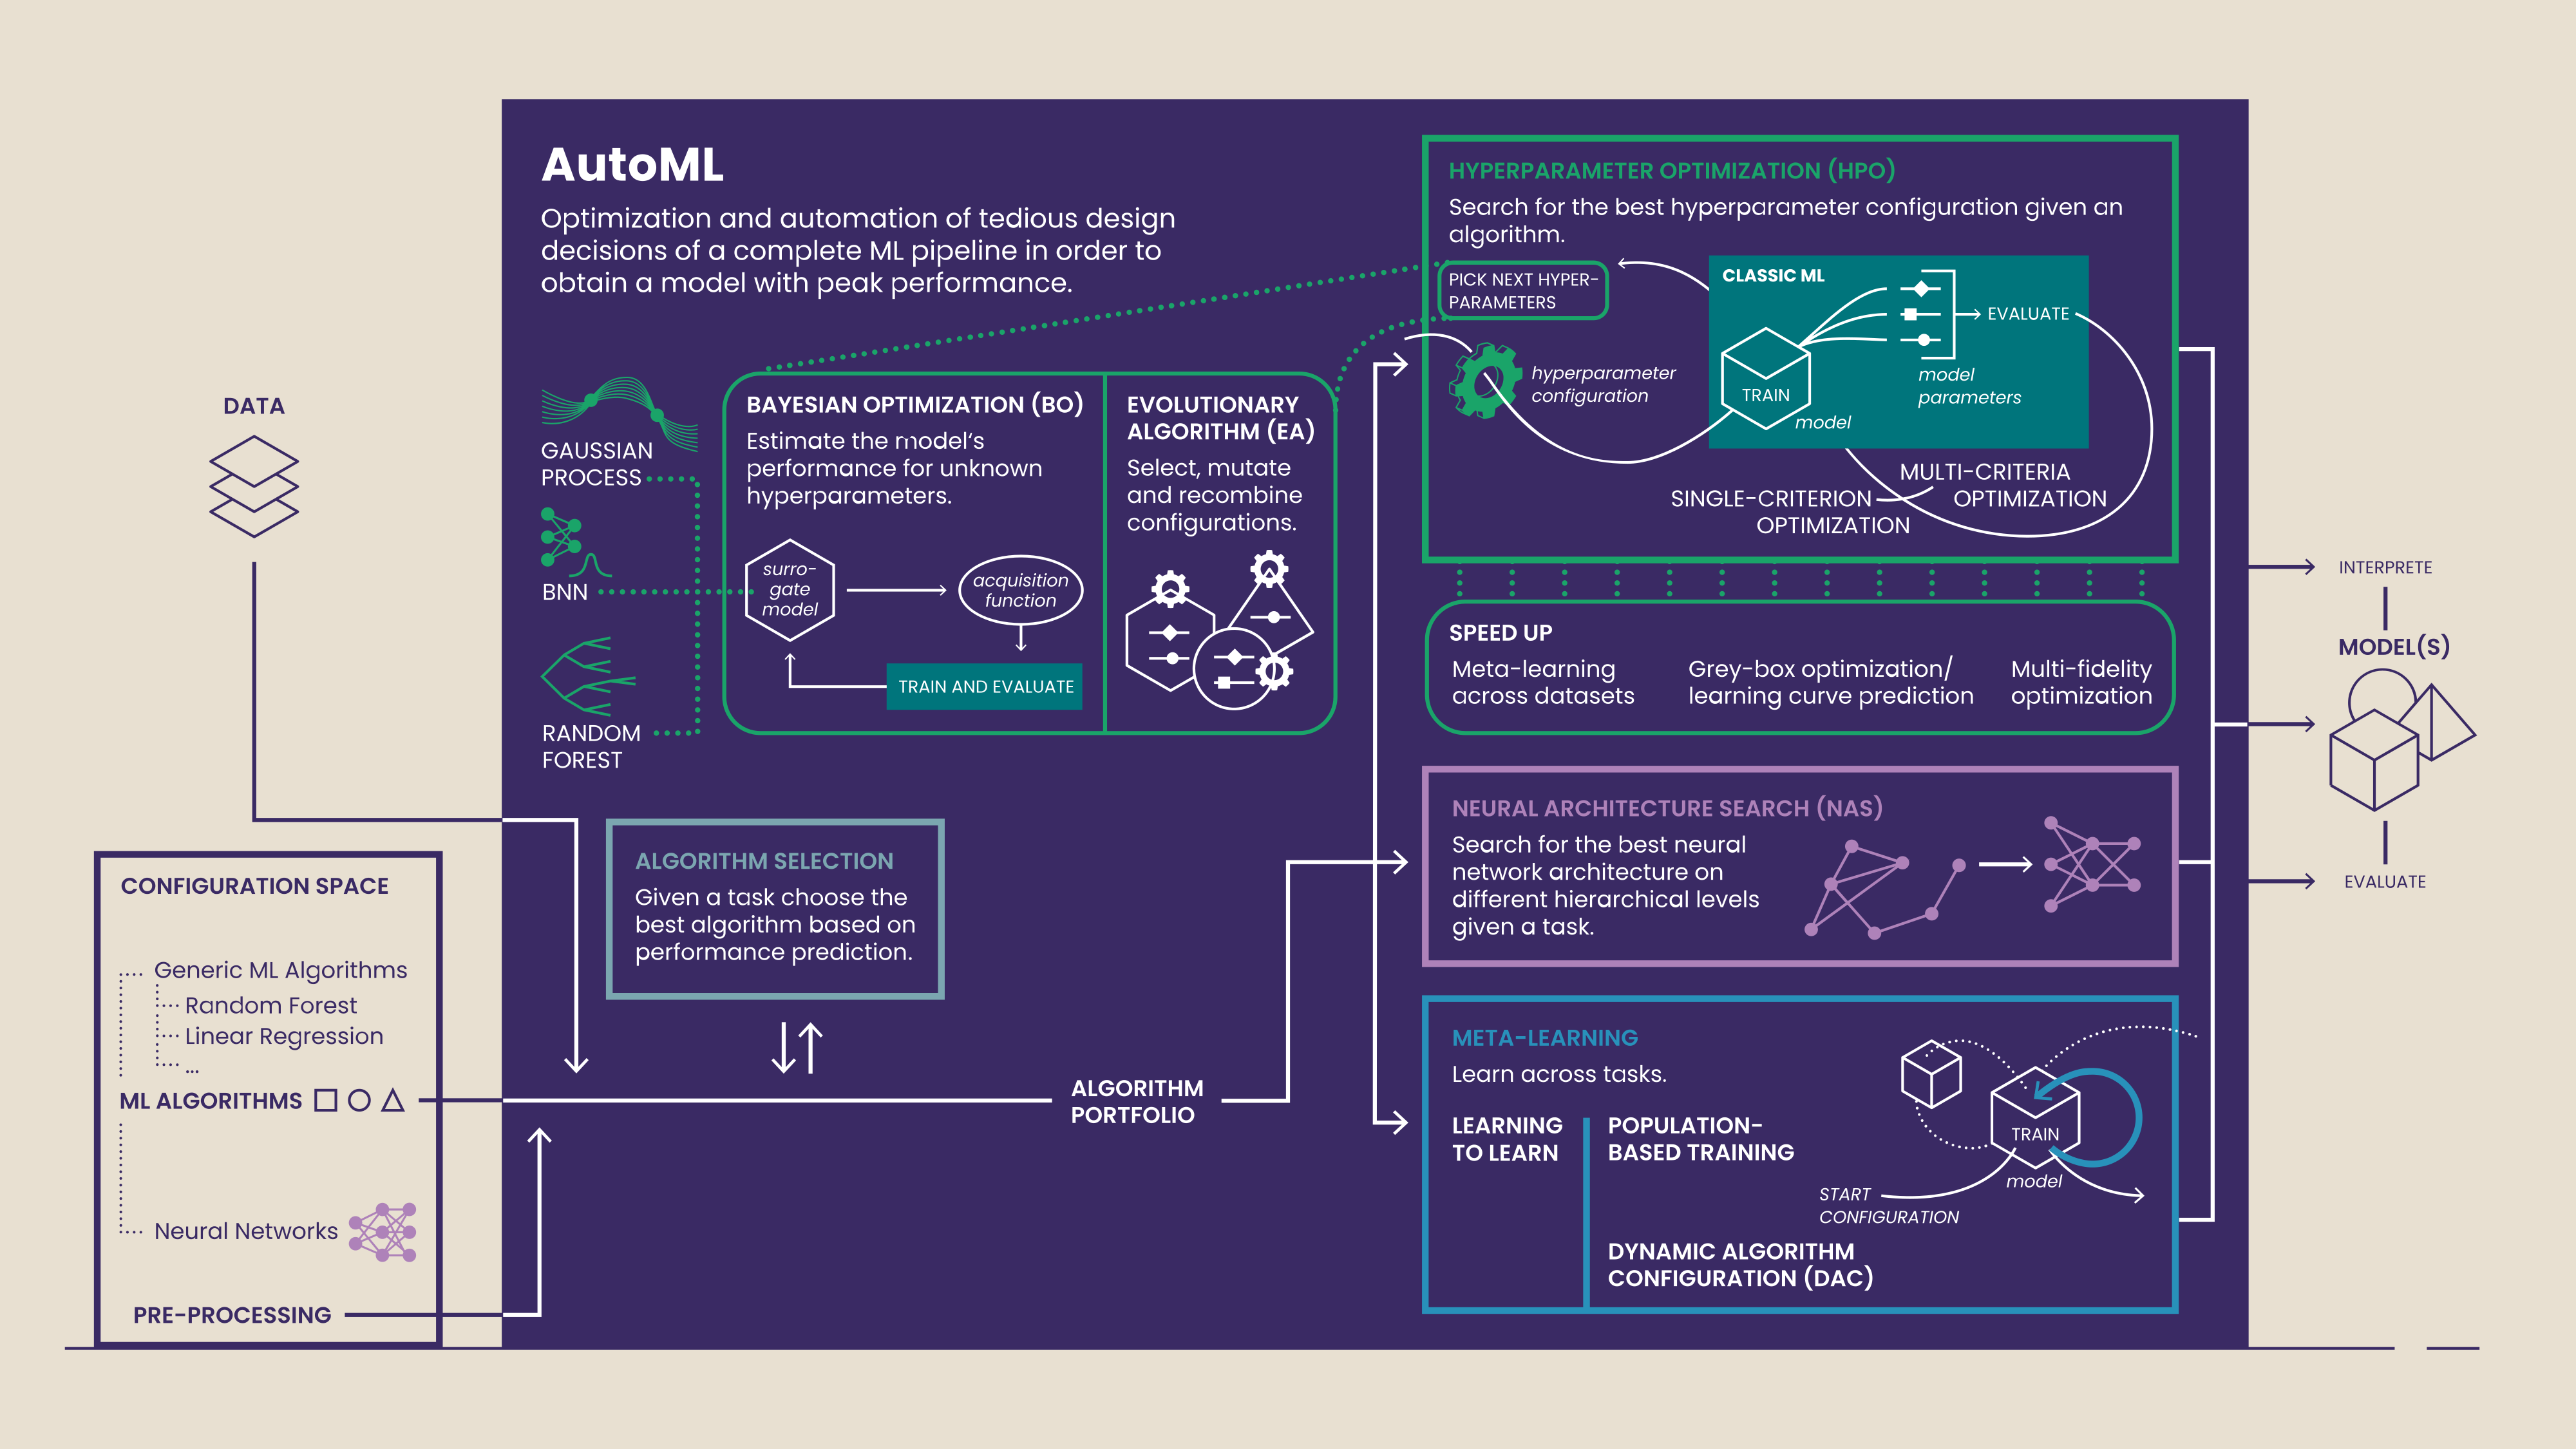
\includegraphics[width = 0.9\linewidth]{images/18_AutoML-Components-Overview-Infographic_corrected.png}  
    \end{center}
\end{frame}

\begin{frame}{What is missing?}
  \begin{columns}
    \begin{column}{0.5\textwidth}
        What do I need to know as an AutoML user?
        \begin{itemize}
          \item \sout{Nothing, because it is automatic.}
          \item Understand limitations of AutoML and framework.
          \item Know how to interpret the results.
          \item Maybe: Data cleaning and feature extraction.
        \end{itemize}

        \vspace{1em}

        Ingredients to implement an AutoML system?
        \begin{itemize}
          \item HPO algorithm
          \item ML / Pipeline framework 
          \item Parallelization / Multi-fidelity
          \item Process encapsulation and time capping 
          \item ...
          % \item (Preprocessing)
        \end{itemize}
    \end{column}%
    \begin{column}{0.5\textwidth}
      \begin{center}

        Practitioners view:
        \scalebox{0.45}{
          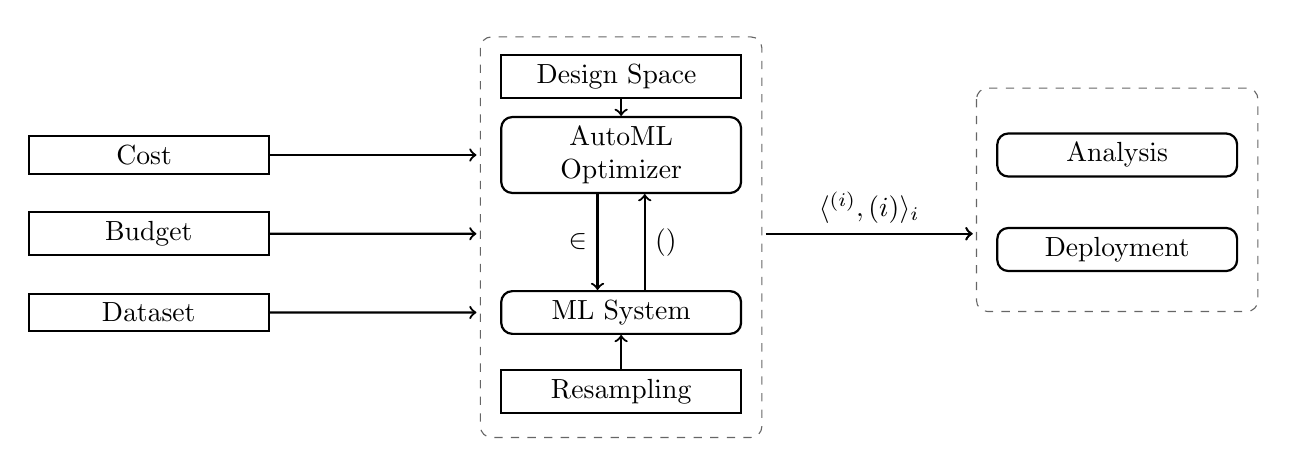
\begin{tikzpicture}[node distance=4cm, thick]
  \node (function) [data] {Cost $\cost$};
  \node (budget) [data, below of=function, node distance=1cm] {Budget};
  \node (dataset) [data, below of=budget, node distance=1cm] {Dataset};
  
  \node (hb) [activity, right of=dataset, node distance=6cm, yshift=-0.0cm] {ML System};
  \node (kde) [activity, above of=hb, node distance=2cm] {AutoML Optimizer};
  \node (resampling) [data, below of=hb, node distance=1cm] {Resampling};
  \node (space) [data, above of=kde, node distance=1cm] {Design Space $\pcs$};
  
  \draw[myarrow] ($(kde.south)+(-0.3,0.0)$) -- ++(0.0,-0.6) node[left] {$\conf \in \pcs$} -- ($(hb.north)+(-0.3,+0.0)$);
  \draw[myarrow] ($(hb.north)+(0.3,+0.0)$) -- ++(0.0,0.6) node[right] {$\cost(\conf)$} -- ($(kde.south)+(0.3,0.0)$);
  
  \draw[myarrow] (function.east) -- ($(kde.west)+(-0.3,0.0)$);
  \draw[myarrow] (budget.east) -- ($(kde.west)+(-0.3,-1.)$);
  \draw[myarrow] (dataset.east) -- ($(kde.west)+(-0.3,-2.)$);

  \draw[myarrow] (space.south) -- ($(kde.north)+(-0.0,0.0)$);
  \draw[myarrow] (resampling.north) -- ($(hb.south)+(-0.0,0.0)$);
  
  \node (perf) [activity, right of=kde, node distance=6.3cm] {Analysis};
  \node (budget) [activity, below of=perf, node distance=1.2cm] {Deployment};
  %\node (imp) [activity, below of=budget, node distance=1cm] {Space Analysis};
  
  \draw[myarrow] ($(kde.east)+(0.3,-1.)$) -- node[above] {$\langle \conf^{(i)}, \cost(\confI{i}) \rangle_i$} ($(perf.west)+(-0.3,-1.)$);
  \draw[myarrow] ($(kde.east)+(0.3,-1.)$) -- node[below] {$\finconf$} ($(perf.west)+(-0.3,-1.)$);
  
  \begin{pgfonlayer}{background}
  
  % Configuration Process
  \path (space -| space.west)+(-0.25,0.5) node (resUL) {};
  \path (resampling.east |- resampling.south)+(0.25,-0.3) node(resBR) {};
  \path [rounded corners, draw=black!60, dashed] (resUL) rectangle (resBR);
  \path (resampling.east |- resampling.south)+(-.5,-.15) node [text=black!60] {};
  
  \path (perf -| perf.west)+(-0.25,0.85) node (resUL) {};
  \path (budget.east |- budget.south)+(0.25,-0.5) node(resBR) {};
  \path [rounded corners, draw=black!60, dashed] (resUL) rectangle (resBR);
  \path (budget.east |- budget.south)+(-.5,-.3) node [text=black!60] {};
  
  \end{pgfonlayer}

\end{tikzpicture}
        }
        \vspace{1em}

        Academic view:
        \scalebox{0.45}{
          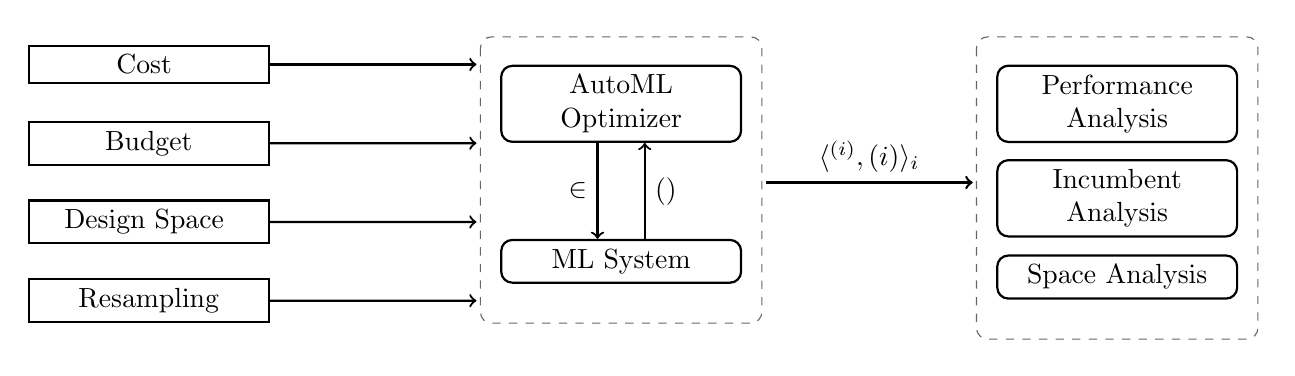
\begin{tikzpicture}[node distance=4cm, thick]
	\node (function) [data] {Cost $\cost$};
	\node (budget) [data, below of=function, node distance=1cm] {Budget};
	\node (space) [data, below of=budget, node distance=1cm] {Design Space $\pcs$};
  \node (resampling) [data, below of=space, node distance=1cm] {Resampling};
	
	\node (hb) [activity, right of=space, node distance=6cm, yshift=-.5cm] {ML System};
	\node (kde) [activity, above of=hb, node distance=2cm] {AutoML Optimizer};
	
	\draw[myarrow] ($(kde.south)+(-0.3,0.0)$) -- ++(0.0,-0.6) node[left] {$\conf \in \pcs$} -- ($(hb.north)+(-0.3,+0.0)$);
	\draw[myarrow] ($(hb.north)+(0.3,+0.0)$) -- ++(0.0,0.6) node[right] {$\cost(\conf)$} -- ($(kde.south)+(0.3,0.0)$);
	
	\draw[myarrow] (function.east) -- ($(kde.west)+(-0.3,0.5)$);
	\draw[myarrow] (budget.east) -- ($(kde.west)+(-0.3,-0.5)$);
	\draw[myarrow] (space.east) -- ($(kde.west)+(-0.3,-1.5)$);
  \draw[myarrow] (resampling.east) -- ($(kde.west)+(-0.3,-2.5)$);
	
	\node (perf) [activity, right of=kde, node distance=6.3cm] {Performance Analysis};
	\node (budget) [activity, below of=perf, node distance=1.2cm] {Incumbent Analysis};
	\node (imp) [activity, below of=budget, node distance=1cm] {Space Analysis};
	
	\draw[myarrow] ($(kde.east)+(0.3,-1.)$) -- node[above] {$\langle \conf^{(i)}, \cost(\confI{i}) \rangle_i$} ($(perf.west)+(-0.3,-1.)$);
	\draw[myarrow] ($(kde.east)+(0.3,-1.)$) -- node[below] {$\incumbent$} ($(perf.west)+(-0.3,-1.)$);
	
	\begin{pgfonlayer}{background}
	
	% Configuration Process
	\path (kde -| kde.west)+(-0.25,0.85) node (resUL) {};
	\path (hb.east |- hb.south)+(0.25,-0.5) node(resBR) {};
	\path [rounded corners, draw=black!60, dashed] (resUL) rectangle (resBR);
	\path (hb.east |- hb.south)+(-.5,-.1) node [text=black!60] {};
	
	\path (perf -| perf.west)+(-0.25,0.85) node (resUL) {};
	\path (imp.east |- imp.south)+(0.25,-0.5) node(resBR) {};
	\path [rounded corners, draw=black!60, dashed] (resUL) rectangle (resBR);
	\path (imp.east |- imp.south)+(-.5,-.2) node [text=black!60] {};
	
	\end{pgfonlayer}

\end{tikzpicture}
        }

      \end{center}
    \end{column}
  \end{columns}
\end{frame}



\end{document}
